\documentclass[a4paper,12pt,french]{book}
\usepackage[T1]{fontenc}
\usepackage[utf8]{inputenc}
\usepackage{graphicx}
\usepackage{calc}

\usepackage[french]{babel}
\usepackage[european, straightvoltages, siunitx]{circuitikz}
\usetikzlibrary{babel}
\ctikzset{inductor=american}

\usepackage{siunitx}

\usepackage{fancyhdr}
\pagestyle{fancy}

% Clear all header and footer fields
\fancyhf{}

% Define the header to include the chapter label
\fancyhead[LE,RO]{\leftmark $~$\rightmark} % Left pages (even): chapter, Right pages (odd): chapter

\newcommand{\e}[1]{\vspace{5mm}\noindent \textbf{\underline{#1}}}

\newcommand{\makeline}{\noindent\makebox[\linewidth]{\rule{\linewidth}{0.4pt}}}

\setcounter{secnumdepth}{-1}

\begin{document}
	
	

\author{Chams GHARIB}
\title{Colles de Physique-Chimie}
\date{2024-2025}

\frontmatter
\maketitle
\tableofcontents

\mainmatter
\chapter{MPSI}
\section{Semaine 01 (16/09-20/09) }


\e{Notions abordées :}
\begin{itemize}
	\item Analyse dimensionnelle.
	\item Circuits électriques dans l'ARQS.
\end{itemize}


\subsection{Questions de cours}

\begin{enumerate}
	\item Définir le courant électrique. Définir l'intensité du courant électrique.
	\item Définir la tension électrique.
	\item Décrire les conventions d'orientation des dipôles. Que valent la puissance reçues et fournies dans chaque cas ?
	\item Qu'est-ce que l'ARQS ? Quelles conséquences ?
	\item Démontrer la formule du pont diviseur de tension.
	\item Démontrer la formule du pont diviseur de courant.
\end{enumerate}

\subsection{Exercice 1 : Application des lois de Kirchoff}

Pour chaque circuit, donner les tensions $u$ et $u_1$ en fonction de $e$ ou bien les intensités $i$ et $i_1$ en fonction de $i_0$.

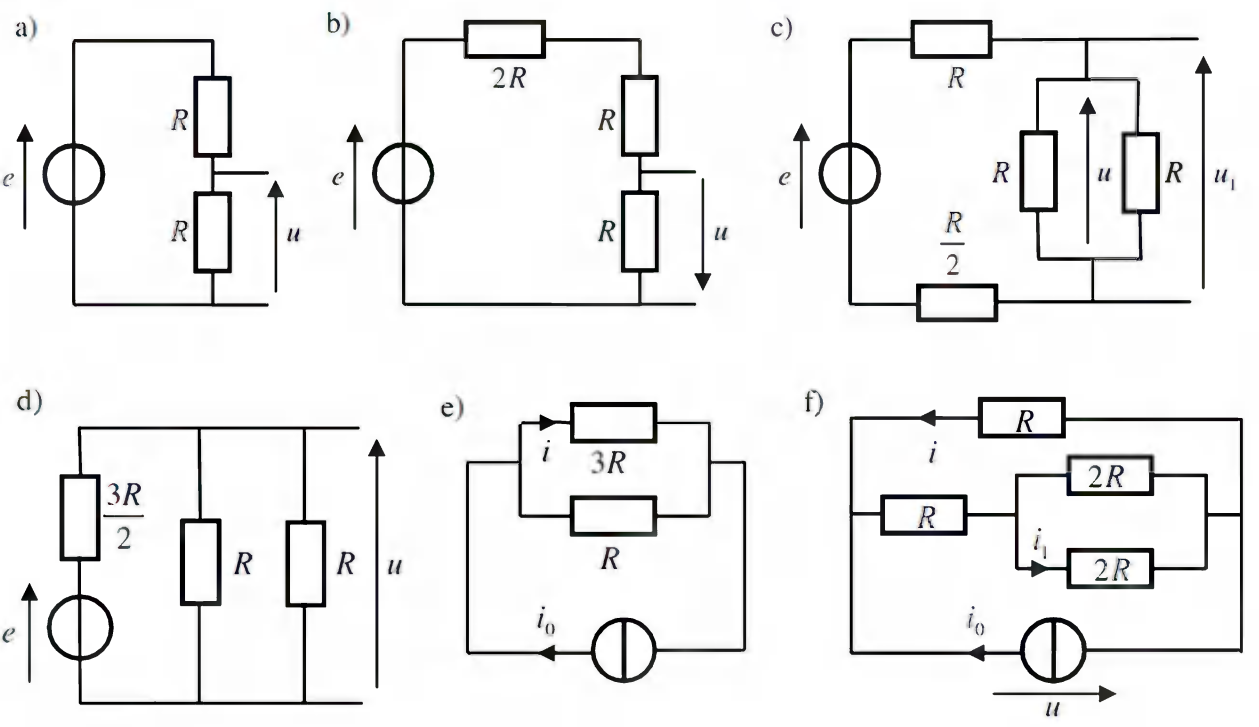
\includegraphics[width=\textwidth]{Images/exercicesKirchoff.png}

\subsection{Exercice 2}

\begin{minipage}[c]{\linewidth/2}
	\begin{circuitikz}
		%Circuit
		\draw (4, 0)
			to[short, i>=$I$] (2, 0)
			to[R, l=$R$] (0, 0)
			to[vsource, v_<=$e$] (0, -3)
			-- (4, -3);
		\draw (2, 0)
			to[R, l_=$R$, v^<=$U$] (2, -3);
	\end{circuitikz}
\end{minipage}%
\begin{minipage}[c]{\linewidth/2}
	On donne $R = \SI{10}{k\Omega}$.
	\begin{enumerate}
		\item Tracer la caractéristique du dipôle ci-contre.
		\item On ajoute une charge de résistance $R'=\SI{3}{k\Omega}$. Déterminer le point de fonctionnement de deux façons.
	\end{enumerate}
\end{minipage}

\subsection{Exercice 3 : Rendement d'un montage potentiométrique}

\begin{minipage}[c]{\linewidth/2}
	\begin{circuitikz}
		%Circuit
		\draw (0, 2)
		to[short, i>=$I$] (0, 3)
		--++(2, 0)
		to[R, l=$r_2$] ++(0, -2)
		to[R, l=$r_1$] ++(0, -2)
		--++(-2, 0)
		--++(0, 1)
		to[vsource, v=$E$] (0, 2);
		\draw (2, 1)
		to[short, i=$i_R$] ++(2, 0)
		to[R, l=$R$] ++(0, -2)
		--++(-2, 0);
	\end{circuitikz}
\end{minipage}%
\begin{minipage}[c]{\linewidth/2}
	Le rendement $\eta$ de ce diviseur de tension est le rapport $P_R$ de la puissance dissipée dans la résistance de charge $R$ à la puissance $P_E$ fournie par la source de tension $E$. Exprimer $\eta$ en fonction de $r_1$, $r_2$ et $R$.
	
	AN : $r_1 = \SI{750}{\Omega}$, $r_2=\SI{250}{\Omega}$, $R = \SI{80}{\Omega}$. Commentaire.
\end{minipage}

\subsection{Exercice 4 : Adaptation de puissance}

\begin{minipage}[c]{\linewidth/2}
	\begin{circuitikz}
		%Circuit
		\draw (0, 0)
		to[R, l=$R_0$] (3, 0)
		to[R, l=$R$] (3, -3)
		-- (0, -3)
		to[vsource, v=$E$] (0, 0);
	\end{circuitikz}
\end{minipage}%
\begin{minipage}[c]{\linewidth/2}
	Un générateur présente une tension à vide $E$ et une résistance interne $R_0$. On y branche une charge de résistance $R$. Pour quelle valeur de $R$ la puissance dissipée dans la résistance $R$ est elle maximale ? Que vaut alors cette puissance ?
\end{minipage}


\chapter{MPI}

\chapter{MP}
\section{Semaine 01 (16/09-20/09) }


\e{Notions abordées :}
\begin{itemize}
	\item Révisions de MPSI en électronique.
	\item Filtrage d'un signal périodique.
	\item Traitement numérique du signal.
\end{itemize}

\subsection{Exercice 1}

\begin{minipage}[c]{\linewidth/3}
	\begin{circuitikz}
		%Circuit
		\draw (0, 0) 
			to[R, l=$R$] (3, 0)
			to [L, l=$L$, v<=$v_s$] ++ (0, -2)
			-- (0, -2)
			to [open, v=$v_e$] (0, 0);
	\end{circuitikz}
\end{minipage}%
\begin{minipage}[c]{\linewidth/2}
	On donne $R = \SI{1.0}{k\Omega}$ et $L = \SI{10}{mH}$.
	\begin{enumerate}
		\item Quel type de filtre ce circuit permet-il de réaliser ?
		\item Déterminer sa fonction de transfert.
		\item Déterminer les pentes des asymptotes en gain BF et HF.
		\item $v_e$ s'écrit comme somme de trois harmoniques de même amplitude, de même phase à l'origine et de fréquences respectives $f_1 = \SI{100}{Hz}$, $f_2 = \SI{1}{kHz}$ et $f_3 = \SI{100}{kHz}$. Écrire $v_e$ puis $v_s$.
		\item $v_e$ est maintenant un triangle de fréquence \SI{60}{Hz}. Quelle est la forme de $v_s$ ?
	\end{enumerate}
\end{minipage}

\subsection{Exercice 2}

\begin{minipage}[c]{\linewidth/2}
	\begin{circuitikz}
		%Circuit
		\draw (0, 0) 
		to[R, l=$R$] (3, 0)
		to[C, l=$C$] ++(2, 0)
		to [L, l=$L$, v<=$v_s$] ++ (0, -2)
		-- (0, -2)
		to [open, v=$v_e$] (0, 0);
	\end{circuitikz}
\end{minipage}%
\begin{minipage}[c]{\linewidth/2}
	\begin{enumerate}
		\item Quel type de filtre ce circuit permet-il de réaliser ?
		\item Déterminer sa fonction de transfert.
		\item Déterminer les pentes des asymptotes en gain BF et HF. Tracer le diagramme de Bode asymptotique.
		\item $v_e$ s'écrit comme somme de trois harmoniques de même amplitude, de même phase à l'origine et de fréquences respectives $f_1 = \SI{100}{Hz}$, $f_2 = \SI{1}{kHz}$ et $f_3 = \SI{100}{kHz}$. Écrire $v_e$ puis $v_s$.
		\item Ce filtre peut-il avoir un comportement dérivateur ? Intégrateur ?
	\end{enumerate}
\end{minipage}

\subsection{Exercice 3}

\begin{minipage}[c]{\linewidth/2}
	\begin{circuitikz}
		%Circuit
		\draw (0, 0) 
			to[R, l=$R$] (2, 0)
			to[C, l=$C$] ++(2, 0)
			to [R, l=$R$] ++ (0, -2)
			-- (0, -2)
			to [open, v=$v_e$] (0, 0);
		\draw (4, 0)
			-- (6, 0)
			to [C, l=$C$, v<=$v_s$] ++ (0, -2)
			-- (4, -2)
			;
	\end{circuitikz}
\end{minipage}%
\begin{minipage}[c]{\linewidth/2}
	On donne $R = \SI{1.0}{k\Omega}$ et $C = \SI{500}{nF}$.
	\begin{enumerate}
		\item Quel type de filtre ce circuit permet-il de réaliser ?
		\item Déterminer sa fonction de transfert.
		\item Déterminer la bande passante. Définir le facteur de qualité.
		\item $v_e$ s'écrit comme somme de trois harmoniques de même amplitude, de même phase à l'origine et de fréquences respectives $f_1 = \SI{100}{Hz}$, $f_2 = \SI{1}{kHz}$ et $f_3 = \SI{100}{kHz}$. Écrire $v_e$ puis $v_s$.
	\end{enumerate}
\end{minipage}

\backmatter
% bibliography, glossary and index would go here.

\end{document}